% 2021年北京高考数学第13题：正方形网格中的向量
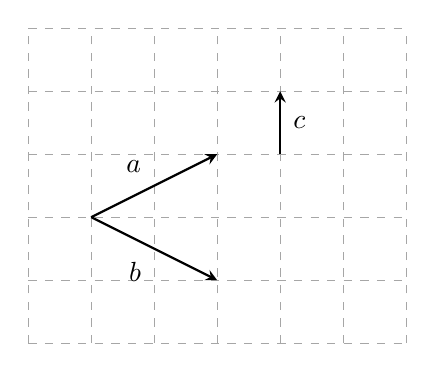
\begin{tikzpicture}[>=stealth,line width=0.6pt,font=\normalsize]
  % 网格
  \draw[dashed,step=0.8cm,gray!70,line width=0.4pt] (0,0) grid (4.8,4.0);

  % 向量
  \coordinate (O) at (0.8,1.6);
  \coordinate (A) at (2.4,2.4);
  \coordinate (B) at (2.4,0.8);
  \coordinate (C1) at (3.2,2.4);
  \coordinate (C2) at (3.2,3.2);

  \draw[->,line width=0.8pt] (O) -- (A) node[midway,above left=1pt] {$\bs a$};
  \draw[->,line width=0.8pt] (O) -- (B) node[midway,below left=1pt] {$\bs b$};
  \draw[->,line width=0.8pt] (C1) -- (C2) node[midway,right=1pt] {$\bs c$};
\end{tikzpicture}
